\chapter{Canonical connection}\label{chap5:chap5}

\setcounter{section}{1}
\setcounter{subsection}{0}


\subsection{}\label{chap5:5.1.1}

\begin{defi*}
By\pageoriginale (\ref{chap4:4.2.2}) an r.m.\@ $(M,g)$ has a canonical
spray $G$. BY 
(\ref{chap2:2.2.3}) there is a unique symmetric connection associated to
$G$. Whenever we consider $(M,g)$ we consider it with the above
connection and refer to $C$ as the {\em connection} or {\em canonical
  connection on} $(M,g)$. Hence given an r.m.\@ $(M,g)$ we can speak
canonically of the concepts associated with a connection, namely, the
derivation law, the curvature tensor, the parallel transport and
Jacobi fields in $(M,g)$.
\end{defi*}

\subsection{}\label{chap5:5.1.2}

\begin{example*}
Now let us examine the connection on $(\mathbb{R}^{d},\epsilon)$. By
\eqref{chap2:2.1.21} it follows that the spray $G'$ associated to the
canonical connection satisfies the equation
\begin{equation*}
\zeta^{T}\circ G'=0.\tag{5.1.3}\label{chap5:5.1.3}
\end{equation*}
By \eqref{chap4:4.2.9} the canonical spray $G$ on
$(\mathbb{R}^{d},\epsilon)$ satisfies the equation
\begin{equation*}
\zeta^{T}\circ G=0.\tag{5.1.4}\label{chap5:5.1.4}
\end{equation*}
We have the direct sum
$T_{z}(T(M))=(\zeta^{T})^{-1}_{z}(0)+(p^{T})^{-1}_{z}(0)$ and since
$p^{T}(G(z))=p^{T}(G'(z))=p'(z)$ we have $G=G'$. Hence by the
uniqueness of the associated symmetric connection we see the canonical
connection on $\mathbb{R}^{d}$ is the same as the connection on
$(\mathbb{R}^{d},\epsilon)$. Now we shall prove that the connection is
carried into the connection by isometries. We know by
(\ref{chap4:4.2.4}) that \pageoriginale the canonical spray is carried
into the canonical spray and we have only to use (\eqref{chap2:2.2.5}).
\end{example*}

\setcounter{subsection}{4}

\subsection{}\label{chap5:5.1.5}

\begin{prop*}
If $(M,g)$ and $(N,h)$ are r.m.'s and
$$
f:(M,g)\to (N,h)
$$
is an isometry, then
$$
(f^{T})^{T}({}^MC(x,y))={}^{N}C(f^{T}(x),f^{T}(y)) \, \forall (x,y)\in
T(M)\mathop{\times}_{M}T(M).  
$$
\end{prop*}

\begin{proof}
By (\ref{chap0:0.4.17}) it is enough to show that both sides of the
equality have the same effect on $d\varphi\in F(T(N))$ for every
$\varphi \in F(N)$. We have
\begin{align*}
&f^{T^{T}}({}^{M}C(x,y))(d\varphi)={}^{M}C(x,y)(d\varphi\circ f^{T})= {}^{M}C(x,y)(d(\varphi\circ f))=\\
&\quad= \frac{1}{2}({}^{M}G(x+y)(d(\varphi\circ
  f))-{}^{M}G(x)(d(\varphi\circ f))-{}^{M}G(y)(d(\varphi\circ f)))=\\
&\quad\hspace{7cm} \text{by (2.2.5)}\\
&\quad= \frac{1}{2}({}^{M}G(x+y)(d\varphi\circ
  f^{T})-{}^{M}G(x)(d\varphi\circ f^{T})-{}^{M}G(d\varphi\circ
  f^{T}))=\\
&\quad=\frac{1}{2}(f^{T})^{T}({}^{M}G(x+y))(d\varphi)-(f^{T})^{T}({}^{M}G(x))(d\varphi)\\
&\qquad{}-(f^{T})^{T}({}^{M}G(y))(d\varphi))=\\
&\quad=\frac{1}{2}({}^{N}G(f^{T}(x+y))(d\varphi)-{}^{N}G(f^{T}(x))(d\varphi)-{}^{N}G(f^{T}(y))(d\varphi))\\
&\quad= {}^{N}C(f^{T}(x),f^{T}(y))(d\varphi)\text{ \ by \ (\eqref{chap2:2.2.5}) and
    since}\\
&\quad\qquad f^{T}(x+y)=f^{T}(x)+f^{T}(y).
\end{align*}
\end{proof}

\subsection{}\label{chap5:5.1.6}

\begin{coro*}
If \pageoriginale $f:(M,g)\to (N,h)$ is an isometry, then 
\begin{itemize}
\item[{\rm i)}] ${}^{N}v\circ (f^{T})^{T}=f^{T}\circ {}^{M}v$

\item[{\rm ii)}] if $S$ is a manifold, $X\in\mathscr{C}(S)$ and
  $\varphi\in D(S,T(M))$, then
  $N_{D_{X}}(f^{T}\circ\varphi)=f^{T}\circ D_{X}$

\item[{\rm iii)}] For every $X_{1}$, $Y_{1}\in\mathscr{C}(M)$
$$
{}^{N}D_{f}T_{\circ X_{1}\circ f^{-1}}(f^{T}\circ Y_{1}\circ
f^{-1})=f^{T}\circ ({}^{M}D_{X_{1}}Y_{1})\circ f^{-1}.
$$
\end{itemize}
\end{coro*}

\begin{proof}
\begin{itemize}
\item[(i)] For every $Z$ in $\mathscr{C}(T(M))$ we have
$$
{}^{M}v\circ Z={}^{M}\xi (Z-C(p'\circ Z,p^{T}\circ Z)).
$$
But from the definition of $\xi$ it follows that the following diagram
is commutative:
\[
\xymatrix@C=.4cm{
 & T_{x}(T_{p(x)}(M))\ar[dl]_{i^{T}_{x}}\ar[dr]^{\zeta_{x}}\ar[ddd]^>>>>>>>>>>>{(f^{T})^{T}} &\\
V_{x}\ar[rr]_<<<<<<<<<<<<<<{M_{\xi}}\ar[ddd]_{(f^{T})^{T}} & & T_{p(x)}(M)\ar[ddd]^{f^{T}}\\
\ar@{}[r] & \ar@{}[r] & \\
 & N_{f^{T}(x)}T_{p(f^{T}(x))}(N)\ar[dl]_{i^{T}_{f^{T}(x)}}\ar[dr]^{\zeta_{f^{T}(x)}}
  &\\
V_{f^{T}(x)}\ar[rr]^-{N_{\xi}} & & T_{p}(f^{T}(x))(N)
}
\]
Hence\pageoriginale
$$
f^{T}\circ {}^{M}\zeta={}^{N}\xi\circ(f^{T})^{T}.
$$
Hence
\begin{align*}
& f^{T}\circ {}^{M}v\circ Z={}^{N}\zeta\circ (f^{T})^{T}\circ
  (Z-C(p'\circ Z, p^{T}\circ Z))=\\
&= {}^{N}\zeta((f^{T})^{T}(Z)-(f^{T})^{T}(C(p'\circ Z,p^{T}\circ
  Z)))=\\
&= {}^{N}\zeta\circ ((f^{T})^{T}\circ Z-C(f^{T}\circ p'\circ
    Z,f^{T}\circ p^{T}\circ Z))\text{ \ by (\ref{chap5:5.1.5})}=\\
&= {}^{N}\zeta((f^{T})^{T}\circ Z-C(p'\circ (f^{T})^{T}\circ Z,
    p^{T}\circ (f^{T})^{T}\circ Z))=\\
&= ^{N}v\circ (f^{T})^{T}\circ Z.
\end{align*}

\item[(ii)] We have
\begin{align*}
& {}^{N}D_{X}(f^{T}\circ\varphi)={}^{N}v\circ
  (f^{T}\circ\varphi)^{T}\circ X\text{ \ by definition, }=\\
& ={}^{N}v\circ (f^{T})^{T}\circ \varphi^{T}\circ X=\\
&= f^{T}\circ {}^{M}v\circ\varphi^{T}\circ X\text{ by (i)} =\\
& f^{T}\circ D_{X}\varphi\text{ \ by the definition of } D_{X}.
\end{align*}

\item[(iii)] We have only to apply (ii) and (\ref{chap2:2.3.14})
\end{itemize}
\end{proof}

\setcounter{subsection}{6}
\subsection{An application.}\label{chap5:5.1.7}
Let $f:(M,g)\to (N,h)$ be an isometry and let $\varphi$ be a curve in
$(M,g)$ and $\psi$ a parallel lift of $\varphi$. Then
${}^{M}D_{P}\psi=0$. Hence by (ii) it follows that $f^{T}\circ \psi$
is a parallel lift of $f\circ\varphi$ in $(N,h)$.

\subsection{}\label{chap5:5.1.8}

\begin{example*}
Let $(G,H)$ be a symmetric pair and $(M,\gamma)$ be an associated
riemannian homogeneous manifold, as in (\ref{chap3:sec3}). Let\pageoriginale
$X\in\underbar{M}$ and let
$$
\varphi:t\to p(\exp(t.X))
$$
be the associated geodesic and $\psi$ a parallel lift of
$\varphi$. Then we {\em claim~:}
$$
\psi(t)=(\tau(\exp(t.X)))^{T}(\psi(0))
$$
i.e. the parallel transport is given by the tangent maps of the one
parameter family of diffeomorphisms induced by $X$.
\end{example*}

\begin{proof}
We know that for every $t_{0}$, $\tau(\exp(t_{0}\cdot X))$ takes the
image of $\varphi$ into itself and is an isometry. Hence
$(\tau(\exp(t_{0}\cdot X)))^{T}$ takes $\psi$ again into a parallel
lift thanks to (\ref{chap5:5.1.7}). But we do not know if it coincides with
$\psi$. On the other hand we know that the map
$\widehat{\sigma}_{\varphi(t_{0})}$ is an isometry and hence preserves
parallel lifts, maps the image of $\varphi$ into itself and further
$(\widehat{\sigma}_{\varphi(t_{0})})^{T}$ is an isometry and acts as
the negative of identity on $T_{(t_{0})}(M)$. Hence $\psi(t)$ goes
into $-\psi(-t)$. Therefore we try to represent $\tau(\exp(tX))$ as
the composition of an even number of symmetries.
\end{proof}

Clearly $(\widehat{\sigma}_{\varphi(t_{0})})^{T}\circ \psi$ is a
parallel lift of $\widehat{\sigma}_{\varphi(t_{0})}\circ\varphi$. But
by (\ref{chap3:3.3.20}) we have
$$
(\widehat{\sigma}_{\varphi(t_{0})}\circ f)(t)=f(2t_{0}-t),
$$

and hence with the notation of (\ref{chap0:sec5})
$$
\widehat{\sigma}_{\varphi(t_{0})}\circ f=f\circ \tau_{2t_{0}}\circ k_{-1}.
$$
Now \pageoriginale consider
$$
\psi_{t_{0}}=-\left(\widehat{\sigma}_{\varphi(t_{0})}\right)^{T}\circ\psi\circ
\tau_{2t_{0}}\circ k_{-1}.
$$
Since $(\tau_{2t_{0}}\circ k_{-1})^{2}=\id_{\mathbb{R}}$, it follows
that $\psi_{t_{0}}$ is a parallel lift of $\psi$ and at $t_{0}$ is
equal to
$$
-\widehat{\sigma}_{\varphi(t_{0})}\circ \psi(t_{0})=\psi(t_{0}).
$$
Hence by the uniqueness of parallel lifts (\ref{chap2:2.7.4}) we have
$$
\psi=\psi_{t_{0}}.
$$
Now if we set $t_{0}=0$ we obtain
$$
\psi=-\widehat{\sigma}^{T}\circ \psi\circ k_{-1}
$$
and hence
$$
\psi=-\widehat{\sigma}_{\varphi(t_{0})}\circ
(-\widehat{\sigma}^{T}\circ \psi\circ k_{-1})\circ \tau_{2t_{0}}\circ
k_{-1}.
$$
But
\begin{gather*}
\widehat{\sigma}_{\varphi(t_{0})}\circ
\widehat{\sigma}=\tau(\exp(2t_{0})X))\text{ \ and hence}\\
\psi=\tau(\exp 2t_{0}X)\circ \psi\circ k_{-1}\circ \tau_{2t_{0}}\circ
k_{-1}\\
=\tau(\exp 2t_{0}X)\circ \psi\circ \tau_{-2t_{0}}\text{ \  since}\\
(\tau_{2t_{0}}\circ k_{-1})^{2}=\id_{\mathbb{R}}.
\end{gather*}
Hence in particular we have
$$
\psi(2t_{0})=(\exp(2t_{0}\cdot X)))^{T}\psi(0).
$$

\section{Riemannian structures on {${{T(M)}}$} and
  {${{U(M)}}$}}\label{chap5:sec2}\pageoriginale

Let $(M,g)$ be an r.m.

For every element $x$ of $T(M)$ the tangent space at $x$ is the direct
sum of $H_{x}$ and $V_{x}$:
$$
T_{x}(T(M))=H_{x}+V_{x}.
$$
The map $\xi$ defines an isomorphism between $V_{x}$ and $T_{p(x)}(M)$
and so does the restriction of $p^{T}$ to $H_{x}$ between $H_{x}$ and
$T_{p(x)}(M)$:
\begin{gather*}
\xi:V_{x}\to T_{p(x)}(M)\\
p^{T}|H_{x}:H_{x}\to T_{p(x)}(M).
\end{gather*}
By means of these isomorphisms and the euclidean structure on\break
$T_{p(x)}(M)$ we define a euclidean structure $\overline{g}$ on
$T_{x}(T(M))$. Precisely:

\subsection{}\label{chap5:5.2.1}

\begin{defi*}
{\em The canonical} r.s.\@ {\em on} $T(M)$, $\overline{g}$, is defined
by the equation
\begin{align*}
\overline{g}(z,z')=g(v(z),v(z'))+g(p^{T}(z),p^{T}(z')) & \; \forall
z,z'\in T_{x}(T(M))\\
&\;\forall x\in T(M).
\end{align*}
\end{defi*}

\subsection{}\label{chap5:5.2.2}

\begin{lemma*}
With respect to this structure $\overline{g}$ for the function $E$ on
$T(M)$ we have (see \ref{chap3:3.6.4}):
$$
\grad (E)=\Xi \in\mathscr{C}(T(M))
$$
where
$$
\Xi(x)=2\xi^{-1}_{x}x, x\in T(M).
$$
\end{lemma*}

\begin{proof}
Let \pageoriginale $Z$ be any vector field on $T(M)$. Then
\begin{align*}
Z(E)=(dE)(Z) &= \overline{g}^{\sharp}(\grad (E))(Z)\tag{5.2.3}\label{chap5:5.2.3}\\
             &= \overline{g}(\grad (E),Z).
\end{align*}
Let $z$ be a horizontal vector. Then we have for $y=p^{T}(z)$:
$$
z=C(x,p^{T}(z))
$$
where $C$ is the canonical connection on $(M,g)$. But by (\eqref{chap2:2.2.5})
and (\ref{chap4:4.3.1}) we have
$$
z(E)=\frac{1}{2}(G(x+y)(E)-G(x)(E)-G(y)(E)).
$$
Hence for every horizontal vector field $Z$ we have
$$
\overline{g}(\grad (E), Z)=0.
$$
Hence $\grad (E)$ is a vertical vector field. Let $x\in T(M)$ and let
$z\in V_{x}$. Then, by (\ref{chap3:3.1.8}) $z(E)=2g(x,\xi(z))$, and by
(\ref{chap5:5.2.1}), since $z$ and $\grad E$ are vertical, we have:
$$
\overline{g}(\grad(E)_{x},z)=g(\xi(\grad(E)),\xi(z)).
$$
Hence by \eqref{chap5:5.2.3} we have
$$
g(2x-\xi(\grad(E)_{x}),\xi(z))=0
$$
for every vertical vector $z$. Since $\xi$ is an isomorphism between
$V_{x}$ and $T_{p(x)}(M)$ and $g$ is non-degenerate we have
$$
2x-\xi(\grad(E)_{x})=0.
$$
Hence:
$$
\grad(E)_{x}=\xi^{-1}_{x}(2x)=2\xi^{-1}_{x}(x).
$$
Since \pageoriginale $U(M)$ is a sub manifold of $T(M)$ there is an
induced r.s.\@ on $U(M)$.
\end{proof}

\setcounter{subsection}{3}

\subsection{}\label{chap5:5.2.4}

\begin{defi*}
The canonical {\em r.s.}\@ $\overline{\overline{g}}$ on $U(M)$ is the
structure $\overline{g}\,|\, U(M)=\overline{\overline{g}}$.
\end{defi*}

\subsection{}\label{chap5:5.2.5}

\begin{prop*}
The volume elements $\overline{\theta}$ and
$\overline{\overline{\theta}}$ of $T(M)$ and $U(M)$ are respectively
given by the equations
$$
\overline{\theta}=|\overline{\sigma}|, \;
\overline{\overline{\theta}}=|\overline{\overline{\sigma}}|  
$$
where
$$
\overline{\sigma}=(-1)^{\frac{d(d-1)}{2}}\cdot \frac{1}{d!}\cdot
\mathop{\wedge}^{d}(d\alpha) 
$$
and 
$$
\overline{\overline{\sigma}}=(-1)^{\frac{d(d-1)}{2}}\cdot
\frac{1}{(d-1)!}\cdot\alpha\wedge(\mathop{\wedge}^{d-1}(d\alpha)). 
$$
\end{prop*}

\setcounter{subsection}{5}
\subsection{}\label{chap5:5.2.6}
Let us note, incidentally, that this implies that $T(M)$ and $U(M)$
are oriented canonically.


\begin{proof}
In view of (\ref{chap3:3.5.1}) and (\ref{chap0:0.3.4}) it is enough to show
that $\overline{\theta}$ and $\overline{\overline{\theta}}$ take value
one on some orthonormal basis of $T_{x}(T(M))$ and $T_{x}(U(M))$ for
$x$ in $T(M)$ and $U(M)$ respectively.
\begin{itemize}
\item[a)] Let us consider $\overline{\theta}$. Let $x\in T(M)$ and let
  $\{x_{1},\ldots,x_{d}\}$ be an orthonormal basis of
  $T_{p(x)}(M)$. Set $p_{i}=\xi^{-1}_{x}x_{i}$ and $z_{i}=C(x,x_{i})$
  $(i=1,\ldots,d)$. Then, by the definition of $\overline{g}$, it
  follows that $\{p_{1},\ldots,p_{d},\unskip\break z_{1},\ldots,z_{d}\}$ is an
  orthonormal basis of $T_{x}(T(M))$. Further by (\ref{chap3:3.6.10}) we
  have
\begin{align*}
& (d\alpha)(p_{i},p_{j})=0\\
& (d\alpha)(p_{i},z_{j})=\delta_{ij} \; \forall i,j\tag{5.2.7}\label{chap5:5.2.7}
\end{align*}\pageoriginale
Hence by the definition of an exterior product through shuffles we have
$$
(-1)^{\frac{d(d-1)}{2}}\mathop{\wedge}^{d}(d\alpha)(p_{1},\ldots,p_{d},z_{1},\ldots,z_{d})=\sum_{\sigma\in P_{d}}\prod^{d}_{i=1}(d\alpha)(p_{\sigma(i)},z_{\sigma(i)})
$$
where $\sigma$ runs through all possible permutations of
$\{1,\ldots,d\}$.\break Hence
$$
(-1)^{\frac{d(d-1)}{2}}\mathop{\wedge}^{d}(d\alpha)(p_{1},\ldots,p_{d},z_{1},\ldots,z_{d})=d!.  
$$

\item[b)] Now let us consider $U(M)$. We want to look at the tangent
  vectors to $U(M)$ among those to $T(M)$. Let us consider the
  injection $i:U(M)\to T(M)$. If $x\in U(M)$ and $z\in T_{x}(T(M))$ is
  a vector in the image of $T_{x}(U(M))$ by $i^{T}$ then there exists
  $z_{1}$ in $T_{x}(U(M))$ such that $i^{T}(z_{1})=z$. But then since
  $E$ is constant on $U(M)$ we have by \eqref{chap5:5.2.3} $0=z_{1}(E\circ
  i)=i^{T}(z_{1})(E)=z(E)=\overline{g}(\grad(E),z)$. Hence every such
  vector $z$ is orthogonal to $\grad(E)$. But the subspace in
  $T_{x}(T(M))$ of vectors orthogonal to $\grad(E)_{x}$ is of
  dimension $2d-1$ which is equal to the dimension of $U(M)$. Since
  $i^{T}_{x}$ is injective we have
\begin{equation*}
i^{T}_{x}(T_{x}(U(M))=\{z|\overline{g}(\grad(E)_{x},z)=0\}.\tag{5.2.8}\label{chap5:5.2.8} 
\end{equation*}
\end{itemize}
\end{proof}

\setcounter{subsection}{8}
\subsection{}\label{chap5:5.2.9}
Now let $x\in U(M)$ and let $\{x_{1},\ldots,x_{d}\}$ be an orthonormal
basis of $T_{p(x)}(M)$ with $x_{1}=x$. Set, as above,
$p_{i}=\xi^{-1}_{x}x_{i}$ and $z_{i}=C(x,x_{i})$ for
$i=1,\ldots,d$. Then, since $\grad(E)_{x}=2\xi^{-1}_{x}$ by
(\ref{chap5:5.2.2}), we see, by \eqref{chap5:5.2.7}, that
$$
\{p_{2},\ldots,p_{d}, z_{1},\ldots,z_{d}\}
$$
is \pageoriginale an orthonormal basis of $T_{x}(U(M))$ and the
relations \eqref{chap5:5.2.7} are valid. Moreover (see \ref{chap3:3.6.6}):
$\alpha(p_{i})=0 \; \forall i$ and $\alpha(z_{1})=g(x_{1},x_{1})=1$. Hence
\begin{align*}
(-1)\frac{d(d-1)}{2}\alpha&\wedge
(\mathop{\wedge}^{d-1}(d\alpha))(p_{2},\ldots,p_{d},z_{1},\ldots,z_{d})\\
&=\sum_{\sigma\in P_{d-1}}\alpha(z_{1})\prod^{d-1}_{i=2}
(d\alpha)(p_{\sigma(i)},z_{\sigma(i)})
\end{align*}
where $\sigma$ runs through all permutations of
$\{2,\ldots,d\}$. Hence
$$
\alpha\wedge(\mathop{\wedge}^{(d-1)}d\alpha)(p_{2},\ldots,p_{d},z_{1},\ldots,z_{d})=(d-1). 
$$
Hence the result.

\subsection{}\label{chap5:5.2.10}
Now let us compute $\vol(U(M),\overline{\overline{g}})$ when $M$ is
compact.

First let us suppose that $M$ is oriented by a form $\sigma_{1}\in
\xi^{d}(M)$, and denote (see (\ref{chap3:sec5})) the canonical orienting form
corresponding to $\sigma_{1}$ by $\sigma$. Let
$\{p_{1},\ldots,p_{d};z_{1},\ldots,z_{d}\}$ be as in the proof (a) of 
(\ref{chap5:5.2.5}). Then we define $\tau\in\xi^{d}(T(M))$ by setting
$$
\tau(p_{1},\ldots,p_{d})=\pm,
$$
according as $\{\xi p_{1},\ldots,\xi p_{d}\}$ is a positive basis of
$T_{m}(M)$ or not, and zero for any other combination from
$\{p_{1},\ldots,p_{d};z_{1},\ldots,z_{d}\}$, and extending,
multilinearly.

First let us note that the restriction of $\tau$ to $T_{m}(M)$ is the
canonical volume form of the euclidean space
$(T_{m}(M),g_{m})$. Then \pageoriginale we have
\begin{equation*}
\overline{\sigma}=(-1)^{\frac{d(d-1)}{2}}\tau\wedge
p^{\ast}_{M}\sigma\tag{5.2.11}\label{chap5:5.2.11} 
\end{equation*}
where $p_{M}:T(M)\to M$. For
\begin{align*}
(\tau\wedge p^{\ast}_{M}\sigma)&(p_{1},\ldots,p_{d},z_{1},\ldots,z_{d})\\
&=\tau(p_{1},\ldots,p_{d})\cdot\sigma(p^{T}(z_{1}),\ldots,p^{T}(z_{d}))=\\
&= \text{1 by the definition of $\tau$.}
\end{align*}
Now let $\{p_{1},\ldots,p_{d},z_{1},\ldots,z_{d}\}$ be as in
(\ref{chap5:5.2.9}). Then define $\omega$ by setting
$\omega(p_{2},\ldots,p_{d})=\pm 1$ according as $\{\xi p_{1},\xi
p_{2},\ldots,\xi p_{d}\}$ is positive or negative with respect to
$\sigma$, and zero for any other combination from
$\{p_{1},\ldots,p_{d},z_{1},\ldots,z_{d}\}$ and extending linearly. We
note that the restriction of $\omega$ to $U_{m}(M)$ is the canonical
volume form on the sphere $(U_{m}(M),\unskip\break g_{m}|U_{m}(M))$ and check (as in
the case of $\tau\wedge p^{\ast}_{M}\sigma)$ that
\begin{equation*}
\overline{\overline{\sigma}}=\omega\wedge
p^{\ast}_{M}\sigma.\tag{5.2.12}\label{chap5:5.2.12} 
\end{equation*}
Now we prove that
\begin{equation*}
\Vol(U(M),\overline{\overline{g}})=\oval{d-1}.\vol
(M,g),\tag{5.2.13}\label{chap5:5.2.13} 
\end{equation*}
{\em where we use the notation}:
\begin{equation*}
\mycirc{d}=\Vol(\mathbb{S}^{d},\epsilon|\mathbb{S}^{d}).\tag{5.2.14}\label{chap5:5.2.14}
\end{equation*}

\begin{proof}
First let us assume that $M$ is oriented. Then $\omega\wedge
p^{\ast}_{M}\sigma$ is a volume form on $U(M)$ and we have
\begin{align*}
\Vol(U(M),\overline{\overline{g}}) &= \int\limits_{U(M)}\omega\wedge
p^{\ast}_{M}\sigma=\\
&=\int\limits_{x\in
  M}\left(\int\limits_{U_{m}(M)}\omega|U_{m}(M)\right)\sigma,\text{
  \ by (\ref{chap0:0.3.17})}
\end{align*}
But\pageoriginale
$$
\int\limits_{U_{m}(M)}\omega|U_{m}(M)=\Vol(\mathbb{S}^{d-1}(T_{m}(M),g_{m}|\mathbb{S}^{d-1}(T_{m}(M)))=\text{(by (\ref{chap0:0.3.15}))}
$$
and because all euclidean structures on vector spaces of the same
finite dimension are isometric, this
$$
=\Vol(\mathbb{S}^{d-1},\epsilon|\mathbb{S}^{d-1})=\oval{d-1}.
$$
Hence
$$
\Vol(U(M),\overline{\overline{g}})=\int\limits_{x\in
  M}\oval{d-1}\; \sigma=\oval{d-1}\cdot \Vol(M,g).
$$

b)~In the general case we take a partition of unity and proceed. Let
$\{W_{i},\varphi_{i}\}$ be a partition of unity on $M$, the $W'_{i}s$
being so small that they can be oriented. Then we have
\begin{equation*}
\sum(\varphi_{i}\circ p)=1\text{ \ on \ } U(M)\tag{5.2.15}\label{chap5:5.2.15}
\end{equation*}
where $p:U(M)\to M$. Now let $\sigma_{i}$ be an orienting form on
$W_{i}$ such that
$$
\overline{\overline{\theta}}|U(W_{i})=|\sigma_{i}|
$$
where
\begin{equation*}
\overline{\overline{\sigma}}_{i}=\omega\wedge(p^{\ast}\sigma_{i}).\tag{5.2.16}\label{chap5:5.2.16} 
\end{equation*}
Then we have
\begin{align*}
& \int\limits_{U(W_{i})}(\varphi_{i}\circ
p)\overline{\overline{\theta}}=\int\limits_{U(W_{i})}(\varphi_{i}\circ
p)\overline{\overline{\sigma}}=\\
&= \int\limits_{U(W_{i})}(\varphi_{i}\circ p)\omega\wedge
p^{\ast}\sigma_{i}.\\
&= \int\limits_{m\in
  W_{i}}\left(\int\limits_{U_{m}(M)}\omega|U_{m}(M)\right)\varphi_{i}|\sigma_{i}|=\oval{d-1}\int\limits_{W_{i}}\varphi_{i}|\sigma_{i}|.\tag{5.2.17}\label{chap5:5.2.17}
\end{align*}
Now\pageoriginale by \eqref{chap5:5.2.17} we have
\begin{align*}
\Vol (U(M),\overline{\overline{g}}) &=
\int\limits_{U(M)}\overline{\overline{\theta}}=\sum_{i}\int\limits_{U(W_{i})}(\varphi_{i}\circ
p)\overline{\overline{\theta}}=\\
&=
\oval{d-1}\sum_{i}\int\limits_{W_{i}}\varphi_{i}|\sigma_{i}|=\oval{d-1}\Vol (M,g).
\end{align*}
\end{proof}

\section{$\Dg=0$}\label{chap5:sec3}

{\em Let us denote the canonical derivation law of the} r.m.\@ $(M,g)$
{\em by} $D$. Since $g\in\mathscr{L}^{2}(M)$ and by \ref{chap2:2.4.7}, we
can introduce the covariant derivative $\Dg\in\mathscr{L}^{3}(M)$. We
shall prove that the 3-form $\Dg$ is zero.

\subsection{}\label{chap5:5.3.1}
First let us note that the form $\Dg$ is symmetric in the last two
variables (because $g$ is symmetric):
\begin{equation*}
\Dg(X,Y,Z)=\Dg(X,Z,Y) \; \forall X,Y,Z\in
\mathscr{C}(M).\tag{5.3.2}\label{chap5:5.3.2} 
\end{equation*}
To start with we shall prove a lemma.

\setcounter{subsection}{2}

\subsection{}\label{chap5:5.3.3}

\begin{lemma*}
$$
\Dg(y,x,x)=2\Dg(x,x,y)\quad \forall (x,y)\in
T(M)\mathop{\times}_{M}T(M).
$$
\end{lemma*}

\begin{proof}
With the notation of (\ref{chap2:sec8}) let us take a one-parameter family
$f$ such that
$$
\uub{P}(0,0)=x, \ \uub{Q}(0,0)=y,
$$
and $f_{0}$ is a geodesic.
\end{proof}

Now let us follow the notations of (\ref{chap4:sec1}). Then since $f_{0}$ is
a geodesic by \eqref{chap4:4.2.1}, and (\ref{chap4:4.1.7}) we have; 
\begin{equation*}
P(\beta(Q))(0,0)=1/2Q(\beta(P))(0,0).\tag{5.3.4}\label{chap5:5.3.4}
\end{equation*}
Further \pageoriginale since the connection is symmetric and $[P,Q]=0$
we have
\begin{equation*}
D_{P}\uub{Q}=D_{Q}\uub{P}\tag{5.3.5}\label{chap5:5.3.5}
\end{equation*}
and since $f_{0}$ is a geodesic
\begin{equation*}
(D_{P}\uub{P})(t,0)=0.\tag{5.3.6}\label{chap5:5.3.6}
\end{equation*}
Further, by the definition of $D$, we have, {\em at the point}
$(t,0)$:
\begin{align*}
P(\beta(Q)) &= P(g(\uub{P},\uub{Q}))\\
            &=
\Dg(\uub{P},\uub{P},\uub{Q})+g(D_{p}\uub{P},\uub{Q})+g(\uub{P},D_{p}\uub{Q})\\ 
            &= \Dg
(\uub{P},\uub{P},\uub{Q})+g(\uub{P},D_{p}\uub{Q})\text{ \  by
  \eqref{chap5:5.3.6}}\\
\text{and}\qquad Q(\beta(P)) &= Q(g(\uub{P},\uub{P}))\\
            &= \Dg(\uub{Q},\uub{P},\uub{P})+2g(D_{Q}\uub{P},\uub{P})\\
            &=
\Dg(\uub{Q},\uub{P},\uub{P})+2g(D_{P}\uub{Q},\uub{P})\text{ \ by \eqref{chap5:5.3.5}.}
\end{align*}
Hence by \eqref{chap5:5.3.4} we have, at the point $(t,0)$
$$
2\Dg(\uub{P},\uub{P},\uub{Q})=\Dg(\uub{Q},\uub{P},\uub{P}),
$$
and hence by the choice of the one parameter family
$$
2 \Dg(x,x,y)=\Dg(y,x,x).
$$
{\em Proof of $\Dg=0$}. Clearly, by the lemma
\begin{equation*}
\Dg(x,x,x)=0\quad \forall x\in T(M).\tag{5.3.7}\label{chap5:5.3.7}
\end{equation*}
Further, we have, by the lemma,
\begin{align*}
&\quad\; \Dg(y,x+y,x+y)=2\Dg(x+y,x+y,y),\\
\text{i.e.}\qquad &\quad\; \Dg(y,x,x)+\Dg(y,y,y)+2\Dg(y,x,y)\\
&= 2\Dg(x,x,y)+2\Dg(x,y,y)+2\Dg(y,x,y)+2\Dg(y,y,y).
\end{align*}
Again by the lemma and \eqref{chap5:5.3.7} we have
\begin{equation*}
\Dg(x,y,y)=0.\tag{5.3.8}\label{chap5:5.3.8}
\end{equation*}\pageoriginale
Hence
\begin{gather*}
\Dg(x,y+z,y+z)=0\\
\text{i.e. \ } \Dg(x,y,y)+\Dg(x,y,z)+\Dg(x,z,y)+\Dg(x,z,z)=0.
\end{gather*}
By (\ref{chap5:5.3.1}) and \eqref{chap5:5.3.8} we have
$$
2\Dg(x,y,z)=0.
$$
Hence
$$
\Dg=0.
$$
Hence we have the following

\setcounter{subsection}{8}

\subsection{}\label{chap5:5.3.9}

\begin{coro*}
\begin{equation*}
X(g(Y,Z))=g(D_{x}Y,Z)+g(Y,D_{x}Z)\; \forall X,Y,Z\text{ \  in
  \ }\mathscr{C}(M).\tag{D.L.5} 
\end{equation*}
\end{coro*}

\section{Consequences of $\Dg=0$}\label{chap5:sec4}
\quad
Now we shall complete the lemma (\ref{chap3:3.6.10}) in the:

\subsection{}\label{chap5:prop5.4.1}

\begin{prop*}
For every $x$ of $T(M)$ we have 
$$
(d\alpha)(z,z')=g(v(z)),p^{T}(z'))-g(v(z'),p^{T}(z)) \; \forall
z,z'\in T_{x}(T(M)).  
$$
\end{prop*}

\begin{proof}
We know that the result holds good if at least one of $z$ and $z'$ is
a vertical vector (see (\ref{chap3:3.6.10})). In view of the bilinearity
of both the sides and the direct sum decomposition 
$$
T_{x}(T(M))=H_{x}+V_{x}
$$
it is enough to prove the result $\forall z$, $z'\in H_{x}$. Now let
$Z$, $Z'\in \mathscr{C}(M)$ be such that 
\begin{equation*}
Z(p(x))=p^{T}(z)\quad\text{and}\quad
Z'(p(x))=p^{T}(z').\tag{5.4.2}\label{chap5:5.4.2} 
\end{equation*}
Then we contend that
$$
d\alpha (Z^{H},{Z'}^{H})=0\quad (\text{see (\ref{chap2:2.5.8})}).
$$
We\pageoriginale have by \eqref{chap0:0.2.10}
\begin{equation*}
d\alpha(Z^{H},{Z'}^{H})=Z^{H}(\alpha({Z'}^{H})-{Z'}^{H}(\alpha(Z^{H})-\alpha([Z^{H},{Z'}^{H}]).\tag{5.4.3}\label{chap5:5.4.3} 
\end{equation*}
But for every $X\in\mathscr{C}(M)$ we have
\begin{align*}
\alpha(Z^{H})\circ X &= g(p'\circ Z^{H}\circ X,p^{T}\circ Z^{H}\circ
X)\\
&= g(X,Z)\text{ \ by (\ref{chap2:2.1.5}) } C_{1}.,
\end{align*}
and hence
\begin{equation*}
\alpha(Z^{H})=g^{\sharp}(Z).\tag{5.4.4}\label{chap5:5.4.4}
\end{equation*}
Now by \eqref{chap5:5.4.4} and \eqref{chap5:5.4.3} we have
\begin{align*}
d\alpha (Z^{H},{Z'}^{H}) &=
Z^{H}(g^{\sharp}(Z'))-{Z'}^{H}(g^{\sharp}(Z))-\alpha([Z^{H},{Z'}^{H}]),\\
&=
D_{Z}(g^{\sharp}(Z'))-D_{Z'}(g^{\sharp}(Z))-\alpha([Z^{H},{Z'}^{H}])\text{
  \ by (\ref{chap2:2.5.9})}.
\end{align*}
Hence for every $X\in\mathscr{C}(M)$ we have
\begin{align*}
d\alpha(Z^{H},{Z'}^{H})\circ X &=
D_{Z}(g^{\sharp}(Z'))(X)-D_{Z'}(g^{\sharp}(Z))(X)-\alpha([Z^{H},{Z'}^{H}]\circ
X)\tag{5.4.5}\label{chap5:5.4.5}\\
&= Z(g(Z',X))-g(Z',D_{Z}X)
\end{align*}
\begin{gather*}
-Z'(g(Z,X))-g(Z,D_{Z'}X)-\alpha([Z^{H},{Z'}^{H}]\circ X)\text{ \ by
  (\ref{chap2:2.4.8})}\\
=g(D_{Z}Z',X)-g(D_{Z},Z,X)-\alpha([Z^{H},{Z'}^{H}]\circ X)\text{ \ by (\ref{chap5:5.3.9}).}
\end{gather*}
But
\begin{align*}
\alpha([Z^{H},{Z'}^{H}]\circ X) &= g(p'\circ [Z^{H},{Z'}^{H}]\circ X,
p^{T}\circ [Z^{H},{Z'}^{H}]\circ X)\tag{5.4.6}\label{chap5:5.4.6}\\
&= g(X,[Z,Z'])\quad \text{(see the proof of (\ref{chap2:2.5.10})).}
\end{align*}
Hence we have by \eqref{chap5:5.4.5} and \eqref{chap5:5.4.6}
\begin{align*}
(d\alpha)(Z^{H},Z^{H})\circ X &= g(D_{Z}Z'-D_{Z'}Z,X)-g(X,[Z,Z'])\\
&= g([Z,Z'],X)-g(X,[Z,Z'])\text{ \  by (\ref{chap2:2.4.1}) D.L.4.}\\
&= 0\text{ \ since $g$ is symmetric.}
\end{align*}\pageoriginale 
This being so for every $X$ we have
$$
(d\alpha)(Z^{H},{Z'}^{H})=0.
$$
Now we shall extend the result (\ref{chap5:5.3.9}). Let $N$ be any
manifold and let $h$, $h'\in D(N,T(M))$ be such that $p\circ h=p\circ
h'$. {\em Then we can define a function $g(h,h')$ on $N$ by setting}
\begin{equation*}
g(h,h')(n)=g(h(n),h'(n)),\quad n\in N.\tag{5.4.7}\label{chap5:5.4.7}
\end{equation*}
Since $h(n)$, $h'(n)\in T_{p(h(n))}(M)$, we have the following result.
\end{proof}

\setcounter{subsection}{7}

\subsection{}\label{chap5:5.4.8}

\begin{coro*}
With the above notation we have
\begin{equation*}
X(g(h,h'))=g(D_{X}h,h')+g(h,D_{X}h')\forall X\in\mathscr{C}(N).\tag{C.D.7}\label{chap5:C.D.7}
\end{equation*}
\end{coro*}

\begin{proof}
This follows directly from (\ref{chap2:prop2.4.7bis}) and $\Dg=0$. 
\end{proof}

\subsection{}\label{chap5:5.4.9}%%till here

\begin{coro*}
Parallel transport preserves $g$.
\end{coro*}

\begin{proof}
Clearly it is enough to prove the result for a curve instead of for a
path. Let $f\in D(I,M)$ be a curve and let $h$ and $h'$ be parallel
lifts of $f$ such that
$$
h(0)=x\quad\text{and}\quad h'(0)=y.
$$
Then we have
\begin{align*}
& \frac{d}{\dt}(g(h(t),h'(t))=P(g(h,h'))=\\
& g(D_{p}h,h')+g(h,D_{p}h')\text{ \ by \ \eqref{chap5:5.4.7}}\\
&= 0\text{ \  since \ } D_{p}h=D_{p}h'=0.
\end{align*}
Hence\pageoriginale $g(h,h')$ is constant on $I$. Hence
$$
g(h(t),h'(t))=g(h(0), h'(0)) \; \forall t\in I.
$$
\end{proof}

\section{Curvature}\label{chap5:sec5}

From the definition of $R$ (see (\ref{chap2:2.5.1})) and from
(\ref{chap5:5.1.6}) iii) it follows, directly, that $R$ is invariant
under isometries, i.e. 

\subsection{}\label{chap5:5.5.1}


\begin{prop*}
If 
$$
f:(M,g)\to (N,h)
$$
is an isometry then $\forall X$, $Y$, $Z\in\mathscr{C}(M)$ we have
$$
f^{T}\circ {}^{M}R(X,Y)Z\circ f^{-1}={}^{N}R(f^{T}\circ X\circ f^{-1},
f^{T}\circ Y\circ f^{-1})(f^{T}\circ Z\circ f^{-1}).
$$
\end{prop*}

\subsection{}\label{chap5:5.5.2}

\begin{remark*}
Let us note that this result in particular implies that an r.m.\@ in
general, is not locally isometric to $\mathbb{R}^{d}$. For, for
$\mathbb{R}^{d}$, $R=0$ by (\ref{chap2:2.5.4}).

Now let us consider the map
\begin{equation*}
(X,Y,Z,T)\to
  g(R(X,Y)Z,T);\mathscr{C}^{4}(M)\to\mathbb{R}\tag{5.5.3}\label{chap5:5.5.3} 
\end{equation*}
and prove
\begin{align*}
g(R(X,Y)Z,T) &= -g(R(X,Y)T,Z)\tag*{(5.5.4) C.T.3}\label{chap5:5.5.4C.T.3}\\
g(R(X,Y)Z,T) &= g(R(Z,T)X,Y)\tag*{(5.5.5) C.T.4}\label{chap5:5.5.5C.T.4}
\end{align*}
\end{remark*}

\begin{proof}
C.T.3. We have by the definition of $R$
\begin{equation*}
g(R(X,Y)Z,Z)=g(D_{X}D_{Y}Z,Z)-g(D_{Y}D_{X}Z,Z)-g(D_{[X,Y]}Z,Z).\tag{5.5.6}\label{chap5:5.5.6} 
\end{equation*}
By by (\ref{chap5:5.3.9}) D.L.5.\@ we have 
\begin{align*}
& g(D_{[X,Y]}Z,Z)=\frac{1}{2}[X,Y](g(Z,Z))\\
& g(D_{X}D_{Y}Z,Z)=X(g(D_{Y}Z,Z))-g(D_{Y}Z,D_{X}Z)\\
\text{and}\qquad & g(D_{Y}D_{X} \,
Z,Z)=Y(g(D_{X}Z,Z))-g(D_{X}Z,D_{Y}Z) 
\end{align*}\pageoriginale
and hence by \eqref{chap5:5.5.6}
\begin{equation*}
g(R(X,Y)Z,Z)=X(g(D_{Y}Z,Z))-Y(g(D_{X}Z,Z))-\frac{1}{2}[X,Y](g(Z,Z));\tag{5.5.7}\label{chap5:5.5.7} 
\end{equation*}
and again by (\ref{chap5:5.3.9})
$$
=X(\frac{1}{2}Yg(Z,Z))-Y(\frac{1}{2}Xg(Z,Z))-\frac{1}{2}[X,Y]g(Z,Z)=0.
$$
Now if we replace $Z$ by $Z+T$ in \eqref{chap5:5.5.7} and carry out the
cancellation we get C.T.3.
\end{proof}

\begin{note*}
We sketch here the geometrical reason for which (C.T.3) holds: because
parallel transport leaves $g$ invariant, and thanks to
(\ref{chap2:2.7.11}), the endomorphism $R(X,Y)$ belongs to the tangent
space of the orthogonal group (i.e.\@ its Lie algebra); this fact is
nothing but (C.T.3).
\end{note*}

\subsection*{C.T.4}
We use C.T.1., C.T.2.\@ and C.T.3.\@ and prove the result
\begin{figure}[H]
\centering
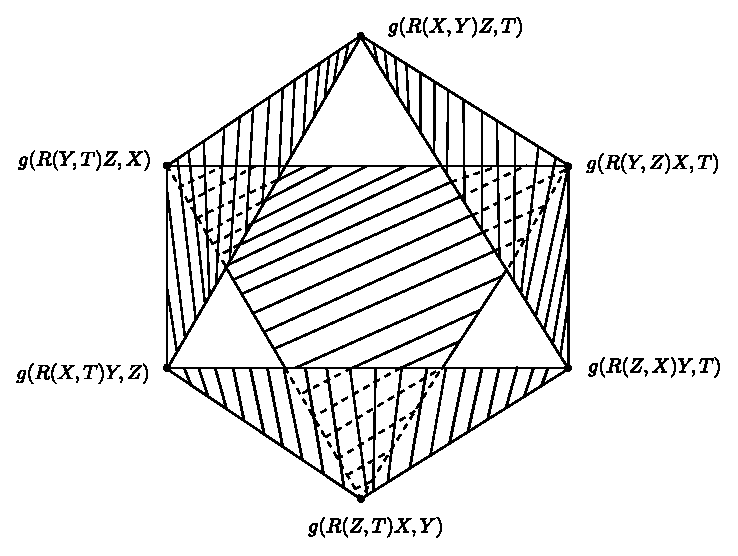
\includegraphics[scale=.75]{figures/chap5-fig1.eps}
\end{figure}

In \pageoriginale the octahedron, the sum of the terms at the three
vertices of every shaded triangle is zero by (C.T.1), (C.T.2) and
(C.T.3). Now adding the terms corresponding to the triangles above and
subtracting the similar sum for the lower ones from it we get
$$
2(g(R(X,Y)Z,T))-2g(R(Z,T)X,Y))=0.
$$

\section{Jacobi fields in an r.m.}\label{chap5:sec6}

Suppose that $f\in D(I,M)$ is a geodesic in an r.m.\@ $(M,g)$ and that
$h$ is a Jacobi field along $f$. Then we have the following
proposition.

\subsection{}\label{chap5:5.6.1}

\begin{prop*}
If for some $t_{0}\in I$,
$$
g(f'(t_{0}),h(t_{0}))=g(f'(t_{0}),(D_{P}h)(t_{0}))=0
$$
then
$$
g(f',h)=0\quad\text{on}\quad I.
$$
\end{prop*}

\begin{proof}
We have
\begin{align*}
\frac{d}{\dt}(g(f',h)) &= P(g(f',h))\tag{5.6.2}\label{chap5:5.6.2}\\
&= g(D_{P}f',h)+g(f',D_{P}h)\text{ \ by \ (\ref{chap5:5.4.8}) (C.D.7)}
=\\
&= g(f',D_{P}h)\text{ \ by \ (\ref{chap2:2.7.3})} 
\end{align*}
and again by (\ref{chap5:5.4.8})  and (\ref{chap2:2.7.3}).
\begin{align*}
\frac{d^{2}}{\dt^{2}}(g(f',h)) &=
\frac{d}{\dt}(g(f',D_{P}h))=\frac{d}{\dt}(g(f',D_{P}h))\tag{5.6.3}\label{chap5:5.6.3}\\
&= g(f',R(f',h)f')\text{ \  by the definition of a}\\
&\qquad \text{of a Jacobi field (see (\ref{chap2:2.8.9}))}\\
&= 0\text{ \  by \ \eqref{chap5:5.5.5C.T.4} C.T.3.}
\end{align*}
Hence
$$
g(f',D_{P}h)\quad\text{is constant on $I$.}
$$
But,\pageoriginale by hypothesis $g(f',D_{P}h)(0)=0$, and hence
$g(f',h)$) is constant on $I$. But $g(f',h)(0)=0$. Hence $g(f,h)=0$.
\end{proof}

\setcounter{subsection}{3}

\subsection{}\label{chap5:5.6.4}

\begin{defi*}
An r.m\@. of dimension two is called a {\em surface}.

As an application of the above proposition we prove the existence of
nice coordinate neighbourhoods for surfaces.
\end{defi*}

\subsection{}\label{chap5:5.6.5}


\begin{application*}
Given a surface $(M,g)$ and a point $m$ of $M$ there exists a chart
$(U,r)$ such that $m$ is in $U$ and if we denote the local coordinates
with respect to $(U,r)$ by $x$ and $y$ then
$$
g|U=dx^{2}+K(x,y)dy^{2}.
$$
\end{application*}

\begin{proof}
Let $\{x_{0},y_{0}\}$ be an orthonormal base of $T_{m}(M)$ and let
$S\in\unskip\break D(J'',M)$ be any curve in $M$ such that
\begin{equation*}
S'(0)=x_{0}\quad\text{and}\quad ||S'(\alpha)||=1.\tag{5.6.6}\label{chap5:5.6.6}
\end{equation*}
\end{proof}

\setcounter{subsection}{6}
\subsection{}\label{chap5:5.6.7}
Then choose the lift $\widetilde{S}(\alpha)$ of $S$ through $y_{0}$
such that at each point $\alpha$, $S'(\alpha)$ and
$\widetilde{S}(\alpha)$ form an orthonormal basis for
$T_{S(\alpha)}(M)$ (see (\ref{chap3:3.1.2})). Now by taking a suitable
sub interval $J'$ of $J''$ and an interval $I$ we can consider the one
parameter family 
\begin{align*}
& f:I\times J'\to M\tag{5.6.8}\label{chap5:5.6.8}\\
& f(t,\alpha)=\exp(t\cdot \widetilde{S}(\alpha)).
\end{align*}
As in the proof of (\ref{chap2:2.8.26}) we get
\begin{equation*}
\begin{split}
& \uub{P}(0,0)=(f^{T}\circ P)(0,0)=x_{0}\\
&\uub{Q}(0,0)=(f^{T}\circ Q)(0,0)=y_{0}
\end{split}\tag{5.6.9}\label{chap5:5.6.9}
\end{equation*}
and hence $f^{T}(0,0)$ is an isomorphism. Therefore by choosing $I$
and $J$ sufficiently small we see, by the inverse function theorem,
that 
\begin{equation*}
f:I\times J\to f(I\times J)=U\tag{5.6.10}\label{chap5:5.6.10}
\end{equation*}\pageoriginale
is a diffeomorphism. Now set
\begin{equation*}
f^{-1}|U=r\tag{5.6.11}\label{chap5:5.6.11}
\end{equation*}
and
\begin{equation*}
x=t\circ r, y=\alpha\circ r.\tag{5.6.12}\label{chap5:5.6.12}
\end{equation*}
Then we have
\begin{equation*}
g|U=g(\uub{P},\uub{P})dx^{2}+2g(\uub{P},\uub{Q})dx\;
dy+g(\uub{Q},\uub{Q})dy^{2}.\tag{5.6.13}\label{chap5:5.6.13}
\end{equation*}
We have
$$
g(\uub{P},\uub{P})(0,\alpha)=||\widetilde{S}(\alpha)||=1\text{ \ by
  the definition of }\widetilde{S}(\alpha)
$$
and 
$$
g(\uub{P},\uub{P})(t,\alpha)=g(\uub{P},\uub{P})(0,\alpha)
$$
by (\ref{chap4:4.3.2}) since for each $\alpha$, $f_{\alpha}(t)$ is a
geodesic, and hence
\begin{equation*}
g(\uub{P},\uub{P})=1.\tag{5.6.14}\label{chap5:5.6.14}
\end{equation*}
Further from the proof of (\ref{chap2:2.8.26}) it follows that for each
$\alpha$
\begin{equation*}
t\to Q(t,\alpha)=h_{\alpha}(t)\tag{5.6.15}\label{chap5:5.6.15}
\end{equation*}
is a Jacobi field along the geodesic $f_{\alpha}(t)$. Further
\begin{align*}
g(f'(0), h_{\alpha}(0) &=
g(\uub{P},\uub{Q})(0,\alpha)\tag{5.6.16}\label{chap5:5.6.16}\\
&= g(\widetilde{S}(\alpha), S'(\alpha))=0
\end{align*}
by our construction; and also
\begin{align*}
g(f'_{\alpha}(0), D_{P}h_{\alpha}(0)) &=
g(\uub{P},D_{P}\uub{Q})(0,\alpha)\tag{5.6.17}\label{chap5:5.6.17}\\
&= g(\uub{P},D_{Q}\uub{P})(0,\alpha)\text{ \  by \ \ref{chap2:2.4.1}
  D.L.4.,}\\
&= g(\widetilde{S},D_{Q}\widetilde{S})(0,\alpha)\\
&=\frac{1}{2}Q(g(\widetilde{S},\widetilde{S}))\text{ \ by
  \ (\ref{chap5:5.4.8})}\\
&= 0\text{ \  by the construction of } \widetilde{S}. 
\end{align*}
Now\pageoriginale (\ref{chap5:5.6.1}) gives that
\begin{equation*}
g(\uub{P},\uub{Q})(t,\alpha)=0 \tag{5.6.18}\label{chap5:5.6.18}
\end{equation*}
Now the result follows if we set $K(x,y)=g(\uub{Q},\uub{Q})$.

\setcounter{subsection}{18}

\subsection{}\label{chap5:5.6.19}

\begin{prop*}
Let $(M,g)$ be an r.m.\@ let $f\in D(I,M)$ be a geodesic and let $h$
be a Jacobi field along $f$. Then
\begin{itemize}
\item[\rm i)] $\dfrac{d(E\circ h)}{\dt}=2g(D_{P}h,h)$

\item[\rm ii]) $\dfrac{d^{2}(E\circ h)}{\dt^{2}}=E\circ
  D_{P}h+g(R(f',h)f',h)$

\item[\rm iii)] if $h(0)=0$ and $(D_{P}h)(0)=y$ with $||y||=1$ then
$$
||h(t)||=t+\dfrac{t^{3}}{6}g(R(f'(0),y)f'(0), y)+0(t^{3}),
$$
where
$$
\dfrac{0(t^{3})}{t^{3}}\to 0\quad\text{with \ }t.
$$
\end{itemize}
\end{prop*}

\begin{proof}
By (\ref{chap5:5.4.8}) we have
\begin{equation*}
\dfrac{d}{\dt}(E\circ h)=P(g(h,h))=2g(D_{P}h,h)\tag{5.6.20}\label{chap5:5.6.20}
\end{equation*}
and again by (\ref{chap5:5.4.8}), we have
\begin{align*}
\dfrac{d^{2}}{\dt^{2}}(E\circ h) &= 2P(g(D_{P}h,h))\\
&= 2g(D_{P}D_{P}h,h)+2g(D_{P}h, D_{P}h)\\
&= 2g(R(f',h)f',h)+2E\circ D_{P}h\text{ \  by the definition (\ref{chap2:2.8.9})}.
\end{align*}
Now \pageoriginale with the notation of \eqref{chap2:2.7.9} by
(\ref{chap2:2.8.18}) we have
\begin{equation*}
\widehat{h}(t)=ty+\dfrac{t^{3}}{6}(R(f'(0),y)f'(0)+0(t^{3})\tag{5.6.21}\label{chap5:5.6.21}
\end{equation*}
and hence
\begin{align*}
||\widehat{h}(t)||^{2} &=
t^{2}g(y,y)+\dfrac{t^{4}}{3}g(R(f'(0),y)f'(0),y)+0(t^{4})\\
&= t^{2}\big(1+\dfrac{t^{2}}{3}g(R(f'(0),y)f'(0),y)+0(t^{2})
\end{align*}
Since $h(t)$ is the parallel transport of $\widehat{h}(t)$ along $f$
we have by (\ref{chap5:5.4.9})
$$
||h(t)||=||\widehat{h}(t)||
$$
Now the rest is the expansion formula for
$$
\sqrt{1+\delta}.
$$
Sometimes it is convenient to re parametrise the arcs by their arc
lengths and then deal with them. In the case of geodesics which are
non trivial this re parametrisation is always possible. Let $f$ be a
geodesic. Then we know that $||f'||$ is constant, by
(\ref{chap4:4.3.2}), say $\theta$. Then $\theta\neq 0$ and for $f\circ
k_{-\theta}$ we have
$$
||(f\circ k_{-\theta})'||=1\quad\text{(see (\ref{chap0:0.5.11})).}
$$
\end{proof}

\setcounter{subsection}{21}
\subsection{}\label{chap5:5.6.22}
Now for any vector $x$ in $U(M)$ {\em let us denote the curve}
$$
t\to \exp(tx)
$$
{\em by} $\gamma_{x}(t)$.

By applying a change of parameter, from (\ref{chap2:2.8.29}) we get the
following result.

\subsection{}\label{chap5:5.6.23}

\begin{prop*}
For every non zero $x$ in $\Omega$ and $y\in
T_{p(x)}(M)$,\pageoriginale we have
$$
\exp^{T}_{m}(\zeta^{-1}_{x}y)=h(||x||)
$$
where $h$ is the Jacobi field along $\gamma_{x/||x||}$ such that
$h(0)=0$ and\break $(D_{P}h)(0)=y/||x||$.
\end{prop*}

\begin{proof}
By (\ref{chap2:2.8.29}) we have
$$
\exp^{T}_{m}(\zeta^{-1}_{x}y)=\overset{\circ}{h} (1)
$$
where $\overset{\circ}{h}$ is the Jacobi field along
$$
\overset{\circ}{f}:t\to \exp (t\cdot x)
$$
such that
$$
\overset{\circ}{h}(0)=0\quad\text{and}\quad (D_{P}\overset{\circ}{h})(0)=y.
$$
But $\gamma\left(\dfrac{x}{x/||x||}\right)=\overset{\circ}{f}\circ
k_{||x||}-1$ and if we set $\overset{\circ}{f}\circ k_{||x||}-1=f$ and
$\overset{\circ}{h}\circ k_{||x||}-1=h$ then $h$ is a Jacobi field
along $f$ such that $h(0)=\overset{\circ}{h}(0)=0$ and
$h(||x||)=\overset{\circ}{h}(1)=\exp^{T}_{m}\left(\zeta^{-1}_{x}y\right)$. 

But $D_{P}h=D_{P}(\overset{\circ}{h}\circ
k_{||x||}-1)=||x||^{-1}D_{P}\overset{\circ}{h}$, so that
$$
D_{P}h(0)=||x||^{-1}D_{P}\overset{\circ}{h}=y/||x||.
$$
\end{proof}


\subsection{}\label{chap5:5.6.24}

\begin{gausslemma*}
For every $x$ and $y$ in $T_{m}(M)$ such that
\begin{equation*}
x\neq 0, x\in\Omega\quad\text{and}\quad g(x,y)=0\tag{5.6.25}\label{chap5:5.6.25}
\end{equation*}
we have
$$
g(\exp^{T}_{m}(\zeta^{-1}_{x}x),\exp^{T}_{m}(\zeta^{-1}_{x}y))=0.
$$
\end{gausslemma*}

\begin{proof}
Let \pageoriginale $h$ be the Jacobi field along $\gamma_{x/||x||}$
such that $h(0)=0$ and $(D_{P}h)(0)=\dfrac{y}{||x||}$. Then we have
$\gamma'_{x/||x||}(0)=\dfrac{x}{||x||}$ and hence
\begin{align*}
g(\gamma'_{x/||x||},h)(0) &= g\left(\dfrac{x}{||x||},0\right)=0,\\
g(\gamma'_{x/||x||},D_{P}h)(0) &= g\left(\frac{x}{||x||},
\frac{y}{||x||}\right)=0\text{ \ by \eqref{chap5:5.6.25}}.
\end{align*}
\begin{figure}[H]
\centering
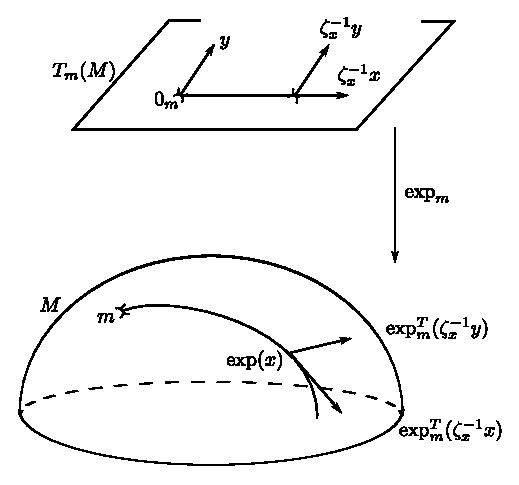
\includegraphics{figures/chap5-fig2.eps}
\end{figure}

\medskip
\noindent
Hence by (\ref{chap5:5.6.1}) we have
\begin{equation*}
g(\gamma'_{x/||x||},h)=0,\tag{5.6.26}\label{chap5:5.6.26}
\end{equation*}
and hence in particular
$$
g(\gamma'_{x/||x||},h)(x)=0.
$$
But by (\ref{chap5:5.6.23}) we have
\begin{equation*}
h(||x||)=\exp^{T}_{m}(\zeta^{-1}_{x}y).\tag{5.6.27}\label{chap5:5.6.27}
\end{equation*}
Further
$$
\gamma_{\frac{x}{||x||}}(t)=\exp\left(t\cdot
  \frac{x}{||x||}\right)=(\exp_{m}\circ S)(t)
$$
where\pageoriginale
$$
S(t)=t\cdot \frac{x}{||x||}.
$$
Hence
$$
\gamma'_{x/||x||}=\exp^{T}_{m}\circ S'.
$$
But
\begin{equation*}
S'(t)=\zeta^{-1}_{\frac{tx}{||x||}}\left(\frac{x}{||x||}\right)\tag{5.6.28}\label{chap5:5.6.28} 
\end{equation*}
and hence
\begin{equation*}
\gamma'_{x/||x||}=\frac{1}{||x||}\exp^{T}_{m}(\zeta^{-1}_{x}x).\tag{5.6.29}\label{chap5:5.6.29} 
\end{equation*}
Now our result follows from \eqref{chap5:5.6.26}, \eqref{chap5:5.6.27} and
\eqref{chap5:5.6.29}.

Now for an $m$ in $M$ and a non zero $x$ in $T_{m}(M)$ set
\begin{align*}
L_{x} &=
\left\{k\zeta^{-1}_{x}x|k\in\mathbb{R}\right\}\tag{5.6.30}\label{chap5:5.6.30}\\
N_{x} &= \left\{\zeta^{-1}_{x}y|g(x,y)=0\right\}.\tag{5.6.31}\label{chap5:5.6.31}
\end{align*}
Then we have the following corollary.
\end{proof}

\setcounter{subsection}{31}

\subsection{}\label{chap5:5.6.32}

\begin{coro*}
With the above notation, we have
\begin{itemize}
\item[\rm i)] $||\exp^{T}_{m}(u)||=||u||$, if $u\in L_{x}$

\item[\rm ii)] $g(\exp^{T}_{m}(L_{x})$, $\exp^{T}_{m}(N_{x}))=0$.
\end{itemize}
\end{coro*}

\begin{proof}
The proof of the first part follows from the fact that $L_{x}$ is one
dimensional and by \eqref{chap5:5.6.29}, (\ref{chap2:2.7.3}) and
(\ref{chap5:5.4.9}). The second part follows from Gauss' lemma.
\end{proof}
